\renewcommand{\thefigure}{\arabic{figure}}

\chapter{Introdução}
\label{ch:introducao}
\begin{resumocapitulo}
Digital Jungle Quest:
Fundada em 2020, a Digital Jungle Quest é uma startup inovadora que oferece uma plataforma de aprendizagem gamificada para auxiliar estudantes universitários e profissionais a aprimorarem suas habilidades digitais.
 \textbf{citação} (\textit{arquivo refs.bib}), \textbf{tabelas}, \textbf{quadros}, \textbf{equações} e \textbf{algoritmos}. Para ter acesso a documentação diretamente na biblioteca da Uninove, \href{http://docs.uninove.br/arte/pdfs/Manual_de_Trabalhos_Academicos_ABNT_UNINOVE.pdf}{clique aqui.}
\end{resumocapitulo}

\chapter{Objetivos}
\label{ch:Objetivos}
Na Digital Jungle Quest, nosso objetivo é ser a bússola que guia os indivíduos em sua jornada pelo ambiente virtual. Comprometemo-nos a fornecer as ferramentas inovadoras, o conhecimento de ponta e o apoio personalizado necessários para que cada aluno possa alcançar seus objetivos educacionais e profissionais. Acreditamos que, com a orientação e os recursos adequados, todos podem concluir seus estudos com confiança e proficiência, preparados para enfrentar os desafios e aproveitar as oportunidades do mundo digital.

\chapter{Sobre Nós}
\label{ch:Sobre Nos}
Sobre Nós
A Digital Jungle Quest nasceu em 2020 com a visão de revolucionar a educação digital. Somos uma startup dedicada a transformar a maneira como jovens alunos e profissionais da área de tecnologia aprendem e desenvolvem suas habilidades. Utilizando uma abordagem gamificada inovadora, nossa plataforma oferece uma experiência de aprendizado envolvente e motivadora, que combina tecnologia de ponta com práticas pedagógicas eficazes.

\begin{figure}
    \centering
    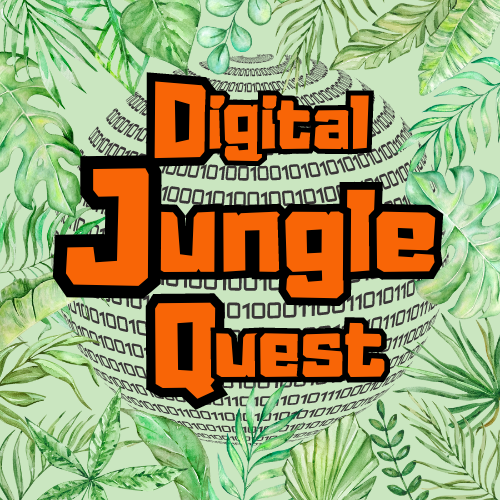
\includegraphics[width=0.75\linewidth]{figuras/DigitalJungleQuestLOGO.png}
    \caption{Digital Jungle Quest LOGO}
    \label{fig:enter-label}
\end{figure}

\chapter{Ideação}
\label{ch:Ideação}
Nossa missão é capacitar a próxima geração de profissionais de tecnologia através de uma educação acessível, interativa e estimulante. Acreditamos que o aprendizado deve ser uma aventura emocionante, repleta de desafios e recompensas que incentivam o progresso contínuo e a aquisição de competências essenciais para o futuro.

Nossa Visão, visualizamos um mundo onde o aprendizado digital é sinônimo de diversão e eficácia. Através da gamificação, queremos criar um ambiente onde os alunos não apenas adquirem conhecimento, mas também desenvolvem habilidades práticas e aplicáveis, essenciais para a carreira na área tecnológica. Nosso objetivo é ser a plataforma líder em educação digital gamificada, reconhecida pela inovação e pelo impacto positivo na formação de profissionais competentes e confiantes.

Nossos Valores

Inovação:
Estamos comprometidos em oferecer soluções educacionais inovadoras que aproveitem as últimas tecnologias e tendências pedagógicas.

Engajamento:
Criamos experiências de aprendizado que mantêm os alunos motivados e engajados, promovendo a retenção e a aplicação prática do conhecimento.

Acessibilidade:
Acreditamos que a educação de qualidade deve ser acessível a todos, independentemente de sua localização ou circunstâncias financeiras.

Excelência:
Buscamos constantemente a excelência em tudo o que fazemos, desde o desenvolvimento de conteúdo até o suporte ao cliente.

Colaboração:
Valorizamos a colaboração e o feedback dos nossos usuários para melhorar continuamente a nossa plataforma e oferecer uma experiência educativa de alta qualidade.

\chapter{Validação da Ideia}
\label{ch:Validacao_da_Ideia}
Na Digital Jungle Quest, acreditamos no poder da inovação e da gamificação para transformar a educação digital. Desde a nossa fundação em 2020, nosso objetivo tem sido criar uma plataforma de aprendizado envolvente e eficaz, destinada a jovens estudantes e profissionais da área de tecnologia. Aqui está como validamos nossa ideia para garantir que estamos atendendo às necessidades de nossos usuários:

Pesquisa de Mercado Inicial
Para entender as necessidades e desafios de nossos potenciais usuários, conduzimos uma pesquisa de mercado abrangente. Realizamos entrevistas detalhadas com estudantes e profissionais de tecnologia para identificar suas dificuldades e preferências no aprendizado digital. Também distribuímos questionários online em fóruns de tecnologia e redes sociais para coletar dados quantitativos. Essa fase inicial foi crucial para identificar o alto interesse por uma abordagem gamificada no aprendizado de habilidades digitais.

Desenvolvimento de um MVP
Com os insights da pesquisa de mercado, desenvolvemos um MVP (Produto Mínimo Viável) que incorporou as funcionalidades essenciais da nossa plataforma. Criamos um protótipo de baixa fidelidade para visualizar a interface e as mecânicas de jogo. Implementamos cursos interativos, quizzes gamificados e um sistema de pontos e recompensas. Este MVP foi lançado para um grupo seleto de usuários em um teste piloto, permitindo-nos obter feedback valioso sobre a usabilidade e o engajamento.

Análise de Dados e Iteração
A análise dos dados de uso e o feedback direto dos usuários do teste piloto foram fundamentais para aprimorar nossa plataforma. Utilizamos ferramentas de análise para monitorar o comportamento dos usuários e identificar áreas de melhoria. Realizamos entrevistas detalhadas e questionários de satisfação para coletar feedback qualitativo. Com base nisso, fizemos ajustes significativos na interface, nas funcionalidades gamificadas e na experiência geral do usuário.

Validação com um Público Maior
Para validar a escalabilidade da nossa plataforma, expandimos o teste para um público maior e mais diversificado. Lançamos um beta público, colaborando com instituições educacionais e empresas de tecnologia para promover a Digital Jungle Quest. Continuamos a coletar feedback contínuo e a realizar atualizações baseadas nas sugestões dos usuários. Essa fase nos permitiu confirmar a viabilidade da plataforma em uma escala maior e identificar oportunidades de crescimento.

Ajustes Finais e Lançamento Oficial
Com os dados e feedback coletados, implementamos as melhorias finais necessárias para preparar a Digital Jungle Quest para o lançamento oficial. Desenvolvemos uma estratégia de marketing robusta para destacar os diferenciais da nossa plataforma gamificada. Estabelecemos um sistema de suporte ao cliente eficiente para atender às necessidades dos novos usuários. Em 2021, lançamos oficialmente a Digital Jungle Quest, proporcionando uma experiência de aprendizado digital inovadora e envolvente.